\section{Additional figures}\label{S:figures}

\begin{figure}[htbp]
\centering
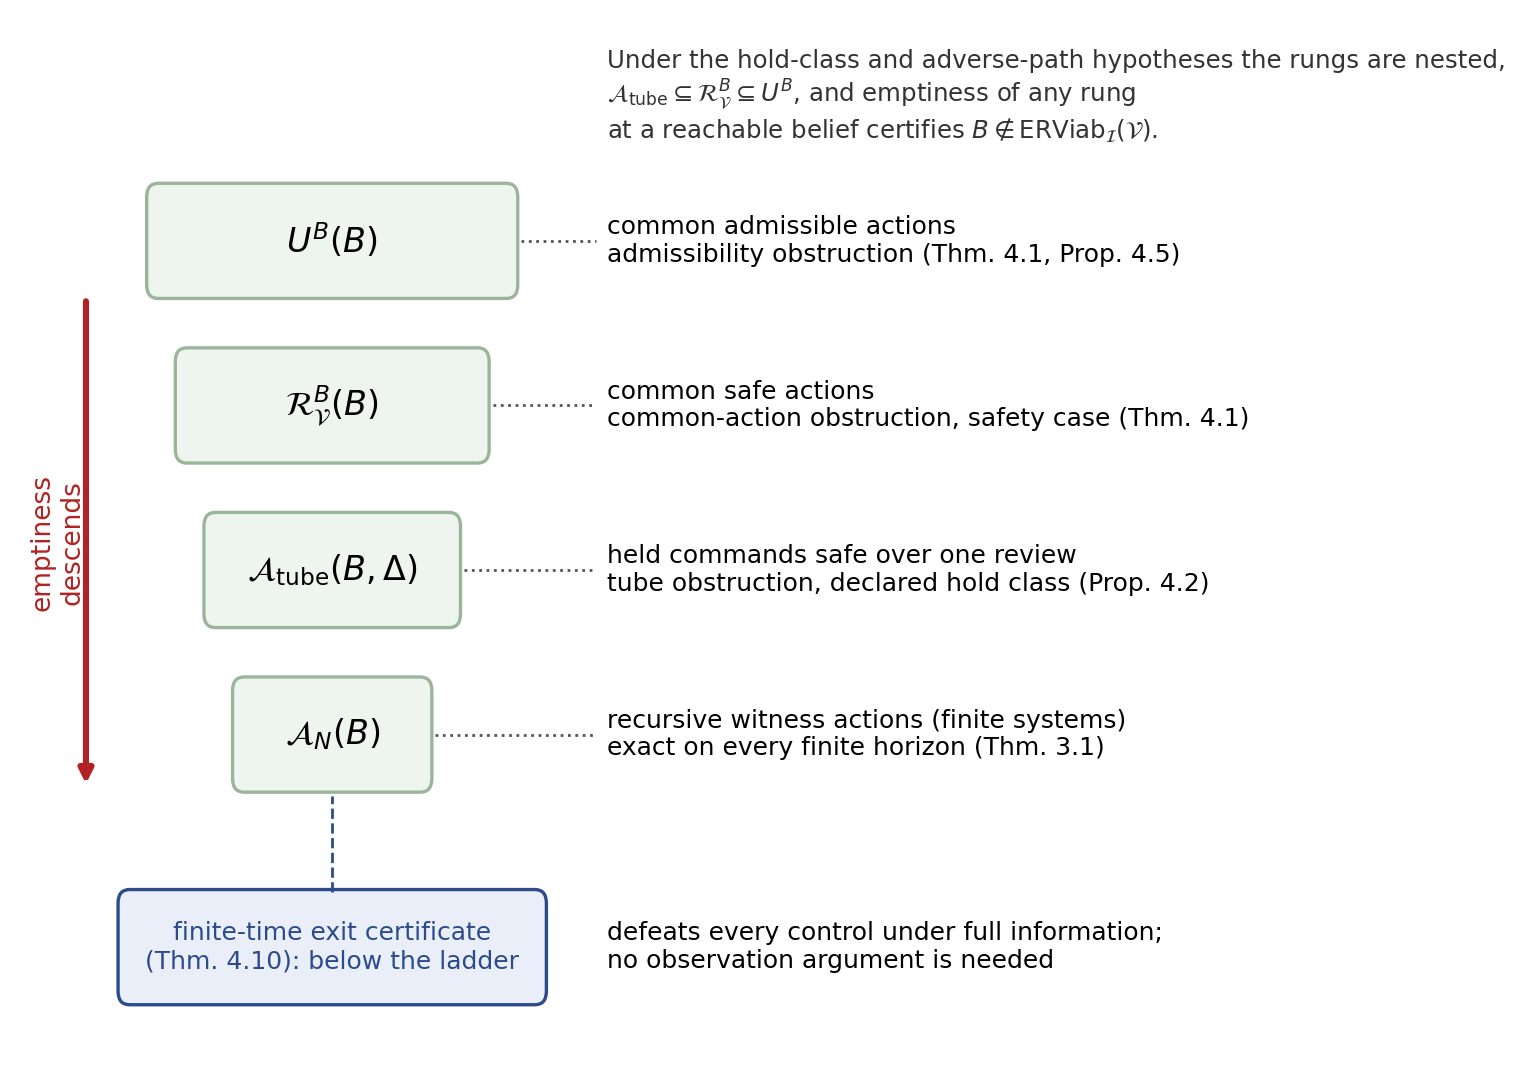
\includegraphics[width=0.9\textwidth]{figs/fig_v73_ladder.png}
\caption{The obstruction ladder (Proposition~4.2). The common response sets are nested, $U^B(B)\supseteq\cR^B_\cV(B)\supseteq\Atube(B,\Delta)$, under the hold-class and adverse-path hypotheses, and emptiness descends; the discrete $\cA_N$ joins the ladder only through a sampled-transition model; the finite-time exit certificate (Theorem~4.10) sits below the ladder because it defeats every control under full information.}
\label{fig:ladder}
\end{figure}

\begin{figure}[htbp]
\centering
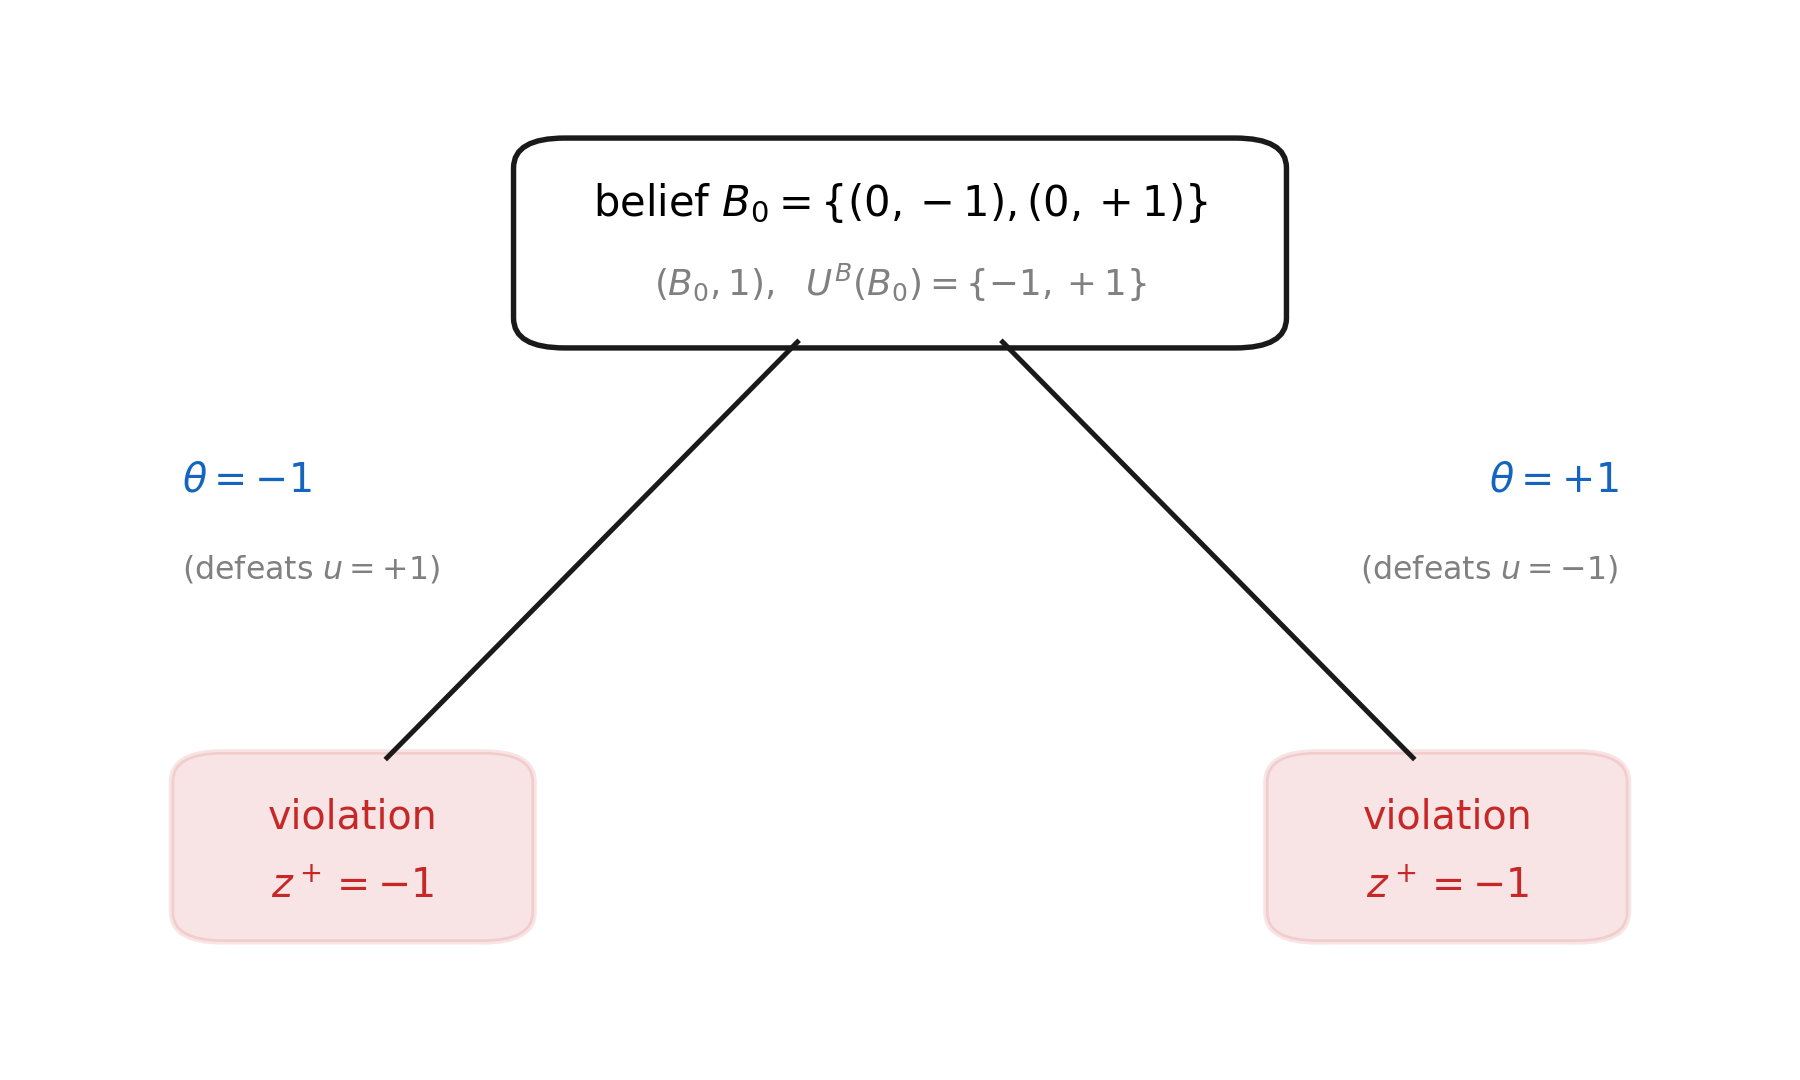
\includegraphics[width=0.62\textwidth]{figs/fig_p2_obstruction_tree.png}
\caption{The one-step obstruction tree of Example~3.3 read as a finite system (\S\ref{S:trees}): for each admissible action the adversary has a compatible branch terminating in violation, so $B_0\notin\cW_1$ (Theorem~3.1); the tree is the Lean term witnessing \texttt{hidden\_mode\_conflict}.}
\label{fig:tree}
\end{figure}

\begin{figure}[htbp]
\centering
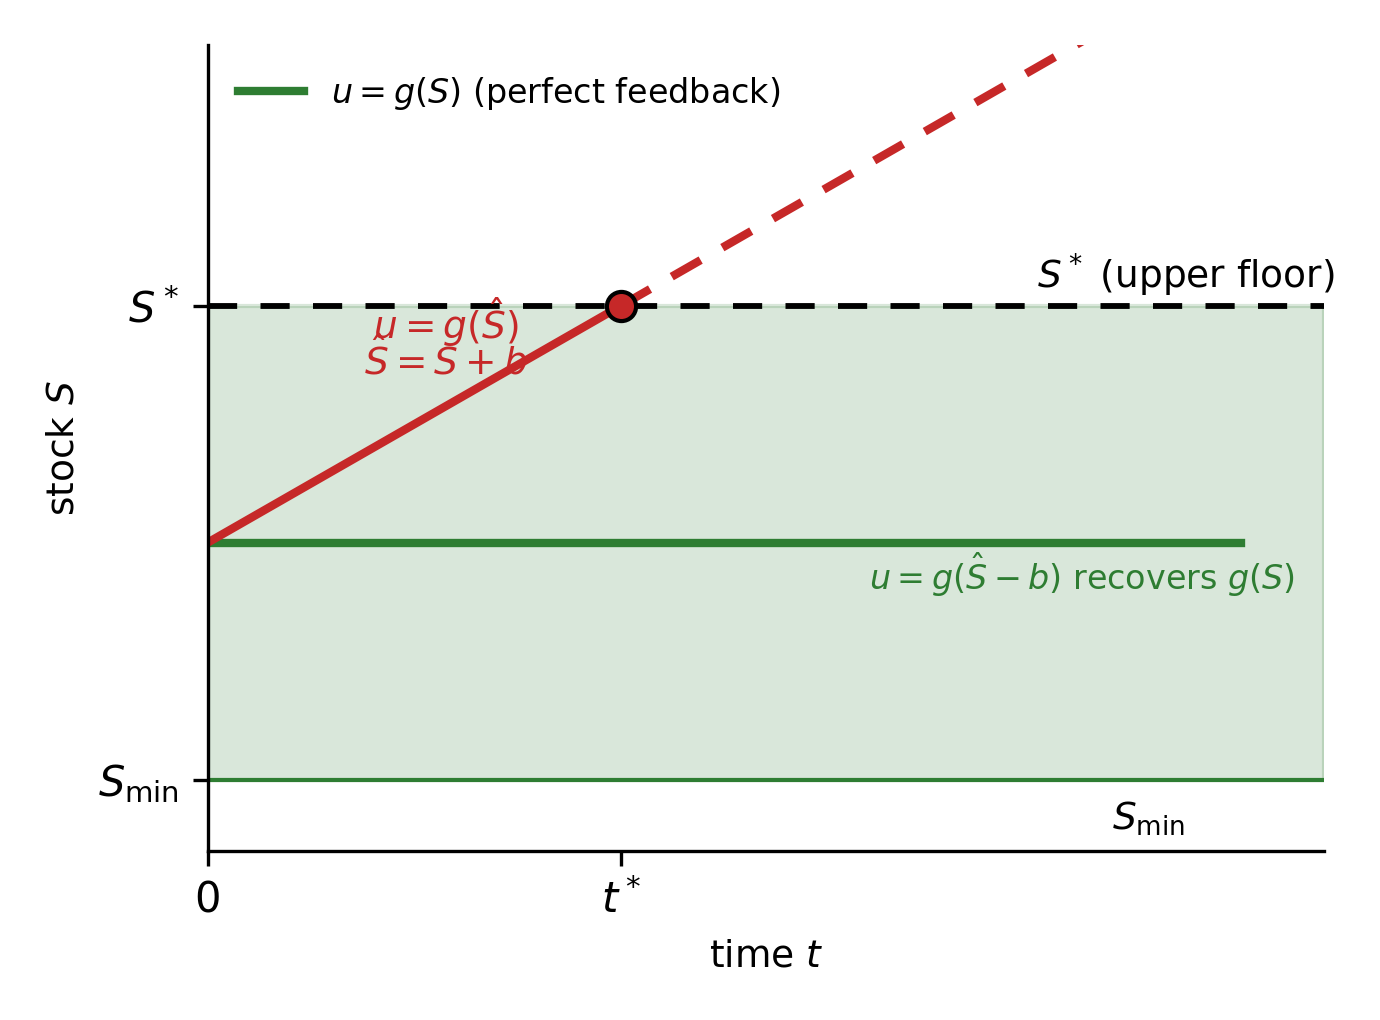
\includegraphics[width=0.6\textwidth]{figs/fig_p2_ce_trap.png}
\caption{The certainty-equivalence trap (Proposition~5.4). Under the perfect-information law $u=g(S)$ the stock is stationary inside $\cV$; the same law applied to the biased observation, $u=g(\hat S)$ with $\hat S=S+b$, gives $\dot S=g(S+b)-g(S)>0$ and exits above $S^*$ in finite time; inverting the bias restores $g(S)$.}
\label{fig:cetrap}
\end{figure}

\begin{figure}[htbp]
\centering
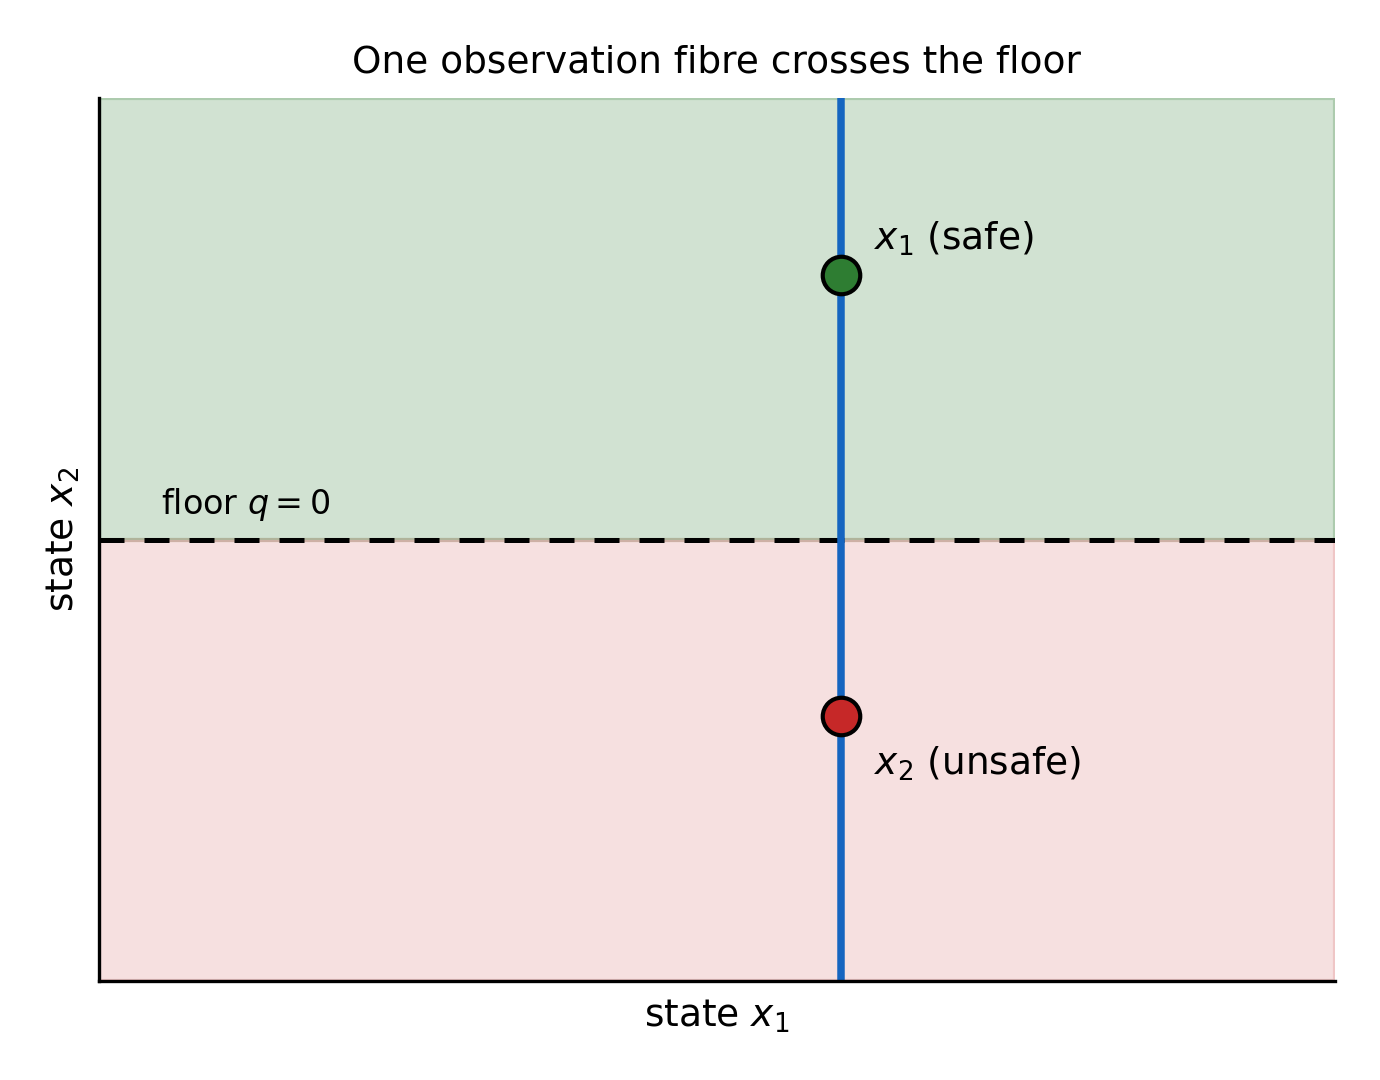
\includegraphics[width=0.72\textwidth]{figs/fig_p2_fibre.png}
\caption{An observation fibre crossing a floor boundary (Proposition~5.2, Corollary~5.3). The observation $O(x)=x_1$ cannot separate the safe state $(0.6,0.8)$ from the unsafe state $(0.6,0.3)$ on the same fibre, so no exact observation-only certifier exists; the certainly-safe readings are those whose entire fibre lies above the floor.}
\label{fig:fibre}
\end{figure}
